\section{RNN Training Setup}
\label{sec:deepspeech:model}

The core of our system is a recurrent neural network (RNN) trained to ingest
speech spectrograms and generate English text transcriptions. Let a single
utterance $x$ and label $y$ be sampled from a training set $\mathcal{X} =
\{(x^{(1)},y^{(1)}),(x^{(2)},y^{(2)}),\ldots\}$. Each utterance, $x^{(i)}$, is
a time-series of length $T^{(i)}$ where every time-slice is a vector of audio
features, $x_t^{(i)}, t=1,\ldots,T^{(i)}$. We use spectrograms as our features,
so $x^{(i)}_{t,p}$ denotes the power of the $p$'th frequency bin in the audio
frame at time $t$. The goal of our RNN is to convert an input sequence $x$ into
a sequence of character probabilities for the transcription $y$, with
$\hat{y_t} = p(c_t \mid x)$, where $c_t \in \{\textrm{a,b,c,}\ldots,\textrm{z},
\textit{space},\textit{apostrophe},\textit{blank}\}$.

Our RNN model is composed of 5 layers of hidden units.  For an input $x$, the
hidden units at layer $l$ are denoted $h^{(l)}$ with the convention that
$h^{(0)}$ is the input. The first three layers are not recurrent. For the first
layer, at each time $t$, the output depends on the spectrogram frame $x_t$
along with a context of $C$ frames on each side.\footnote{We typically use
$C\in \{5, 7, 9\}$ for our experiments.} The remaining non-recurrent layers
operate on independent data for each time step. Thus, for each time $t$, the
first 3 layers are computed by:
\begin{align*}
    h^{(l)}_t &= g(W^{(l)} h^{(l-1)}_t + b^{(l)})
\end{align*}
where $g(z) = \min\{\max\{0,z\}, 20\}$ is the clipped rectified-linear (ReLu)
activation function and $W^{(l)}, b^{(l)}$ are the weight matrix and bias
parameters for layer $l$.\footnote{The ReLu units are clipped in order to keep
the activations in the recurrent layer from exploding; in practice the units
rarely saturate at the upper bound.} The fourth layer is a bi-directional
recurrent layer~\cite{schuster1997bidirectional}. This layer includes two sets
of hidden units: a set with forward recurrence, $h^{(f)}$, and a set with
backward recurrence $h^{(b)}$:
\begin{align*}
    h^{(f)}_t &= g(W^{(4)} h^{(3)}_t + W_r^{(f)} h^{(f)}_{t-1} + b^{(4)}) \\
    h^{(b)}_t &= g(W^{(4)} h^{(3)}_t + W_r^{(b)} h^{(b)}_{t+1} + b^{(4)})
\end{align*}
Note that $h^{(f)}$ must be computed sequentially from $t=1$ to $t=T^{(i)}$ for
the $i$'th utterance, while the units $h^{(b)}$ must be computed sequentially
in reverse from $t=T^{(i)}$ to $t=1$.

The fifth (non-recurrent) layer takes both the forward and backward units as
inputs $h^{(5)}_t = g(W^{(5)} h^{(4)}_t + b^{(5)})$ where $h^{(4)}_t =
h^{(f)}_t + h^{(b)}_t$. The output layer is a standard softmax function that
yields the predicted character probabilities for each time slice $t$ and
character $k$ in the alphabet:
\begin{align*}
    h_{t,k}^{(6)} = \hat{y}_{t,k} \equiv p(c_t = k \mid x) =
        \frac{\exp(W_k^{(6)} h_t^{(5)}+b_k^{(6)})}{\sum_j \exp(W_j^{(6)} h_t^{(5)}+b_j^{(6)})}.
\end{align*}
Here $W_k^{(6)}$ and $b_k^{(6)}$ denote the $k$'th column of the weight matrix
and $k$'th bias, respectively.  

Once we have computed a prediction for $p(c_t \mid x)$, we compute the CTC
loss~\cite{graves2006} $\mathcal{L}(\hat{y}, y)$ to measure the error in
prediction. During training, we can evaluate the gradient $\nabla_{\hat{y}}
\mathcal{L}(\hat{y}, y)$ with respect to the network outputs given the
ground-truth character sequence $y$. From this point, computing the gradient
with respect to all of the model parameters may be done via back-propagation
through the rest of the network. We use Nesterov's Accelerated gradient method
for training~\cite{sutskever2013}.\footnote{We use momentum of 0.99 and
anneal the learning rate by a constant factor, chosen to yield the fastest
convergence, after each epoch through the data.}

\begin{figure}[th]
\centering
 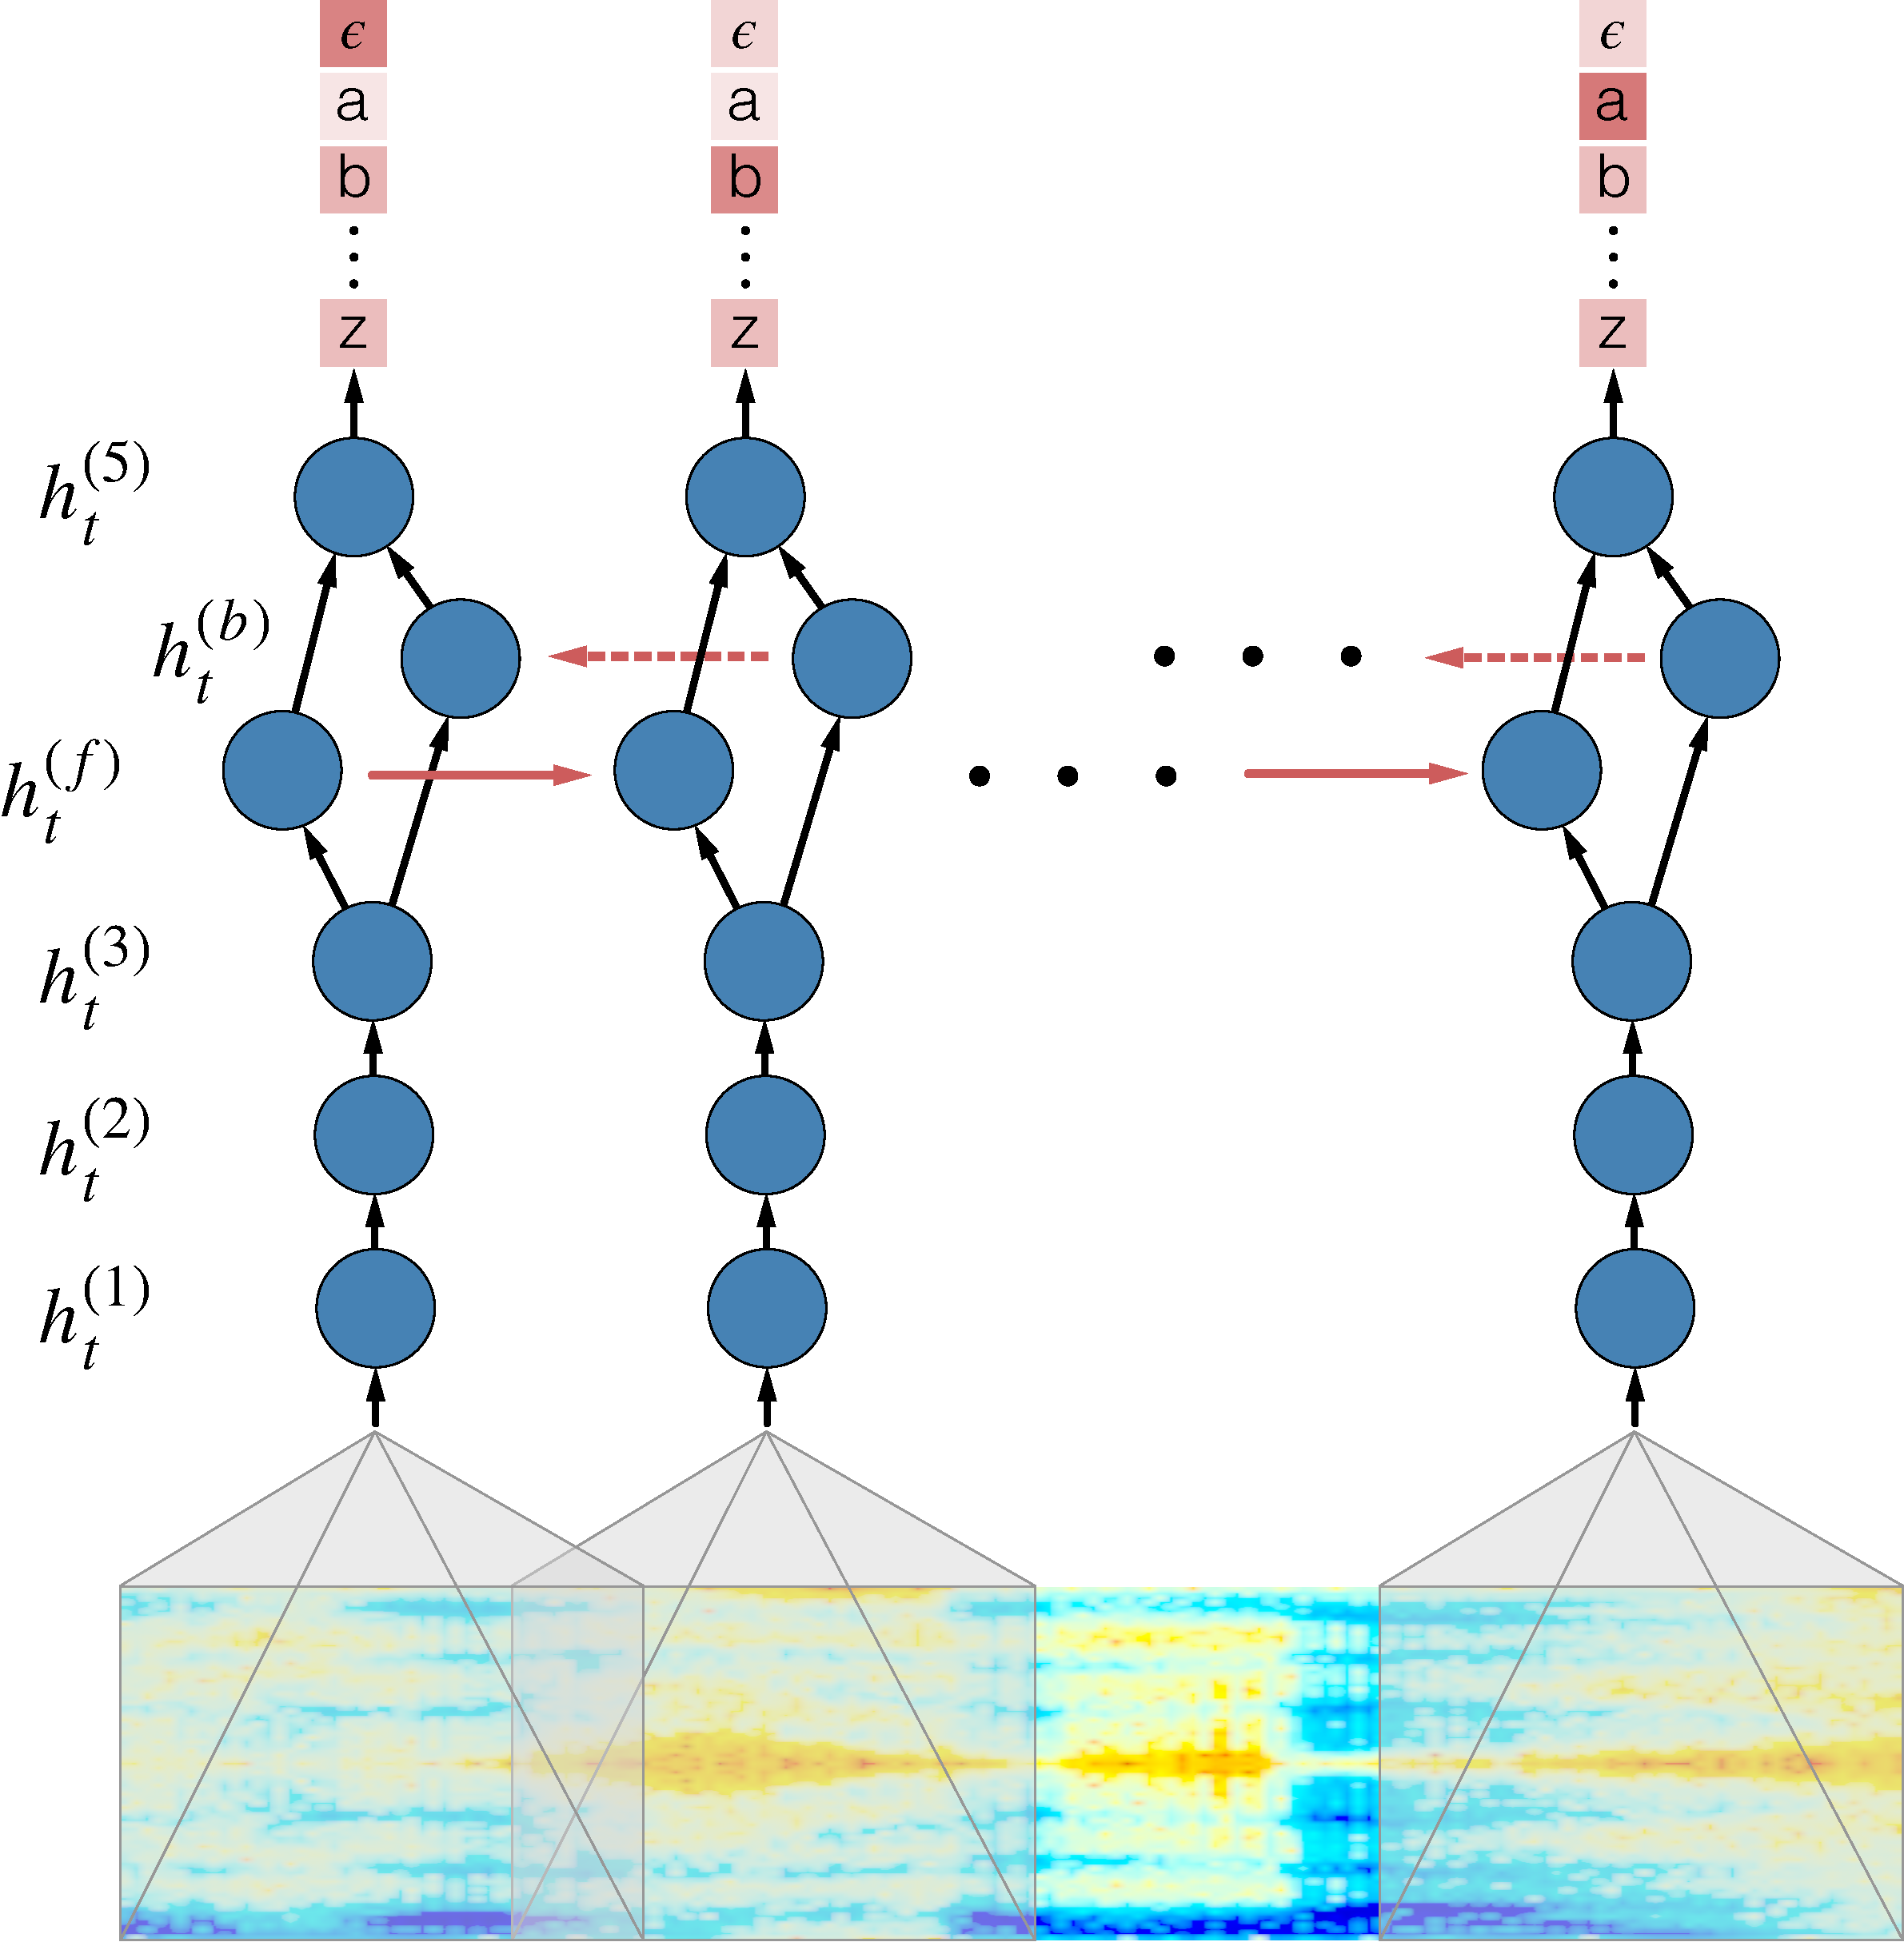
\includegraphics[width=0.6\textwidth]{deepspeech/figures/speech_network.pdf}
  \caption{Structure of our RNN model and notation.}
  \label{fig:deepspeech:rnn}
\end{figure}

The complete RNN model is illustrated in Figure~\ref{fig:deepspeech:rnn}. Note
that its structure is considerably simpler than related models from the
literature~\cite{graves2014}---we have limited ourselves to a single recurrent
layer (which is the hardest to parallelize) and we do not use
Long-Short-Term-Memory (LSTM) circuits. One disadvantage of LSTM cells is that
they require computing and storing multiple gating neuron responses at each
step. Since the forward and backward recurrences are sequential, this small
additional cost can become a computational bottleneck. By using a homogeneous
model we have made the computation of the recurrent activations as efficient as
possible: computing the ReLu outputs involves only a few highly optimized BLAS
operations on the GPU and a single point-wise nonlinearity.

\subsection{Regularization}

While we have gone to significant lengths to expand our datasets (c.f.
Section~\ref{sec:deepspeech:data}), the recurrent networks we use are still
adept at fitting the training data. In order to reduce variance further, we use
several techniques.  

During training we apply a dropout~\cite{hinton2012dropout} rate between 5\% -
10\%. We apply dropout in the feed-forward layers but not to the recurrent
hidden activations.

A commonly employed technique in computer vision during network evaluation is
to randomly jitter inputs by translations or reflections, feed each jittered
version through the network, and vote or average the
results~\cite{krizhevsky2012imagenet}. Such jittering is not common in ASR,
however we found it beneficial to translate the raw audio files by 5ms (half
the filter bank step size) to the left and right, then forward propagate the
recomputed features and average the output probabilities. At test time we also
use an ensemble of several RNNs, averaging their outputs in the same way.

\subsection{Language Model}
\label{sec:deepspeech:languagemodel}

When trained from large quantities of labeled speech data, the RNN model can
learn to produce readable character-level transcriptions. Indeed for many of
the transcriptions, the most likely character sequence predicted by the RNN is
exactly correct without external language constraints. The errors made by the
RNN in this case tend to be phonetically plausible renderings of English
words---Table~\ref{table:deepspeech:max_decoded} shows some examples. Many of
the errors occur on words that rarely or never appear in our training set. In
practice, this is hard to avoid:  training from enough speech data to
\emph{hear} all of the words or language constructions we might need to know is
impractical.  Therefore, we integrate our system with an N-gram language model
since these models are easily trained from huge unlabeled text corpora. For
comparison, while our speech datasets typically include up to 3 million
utterances, the N-gram language model used for the experiments in
Section~\ref{sec:deepspeech:expnoise} is trained from a corpus of 220 million
phrases, supporting a vocabulary of 495,000 words.\footnote{We use the KenLM
toolkit~\cite{heafield2013} to train the N-gram language models in our
experiments.} 

\begin{table}[h]
\centering
\begin{tabular}{l | l}
\toprule
RNN output  & Decoded Transcription \\
\midrule
\rule{0pt}{2ex}
what is the weather like in & what is the weather like in \\
\rule{0pt}{0.1ex}
bostin right now       & boston right now \\
\rule{0pt}{4ex}
prime miniter nerenr modi   & prime minister narendra modi \\ 
\rule{0pt}{4ex}
arther n tickets for the game  & are there any tickets for the game \\ 
\bottomrule
\end{tabular}
\caption{Examples of transcriptions directly from the RNN (left) with errors
         that are fixed by addition of a language model (right).}
\label{table:deepspeech:max_decoded}
\end{table}

Given the output $p(c \mid x)$ of our RNN we perform a search to find the
sequence of characters $c_1,c_2,\ldots$ that is most probable according to both
the RNN output and the language model (where the language model interprets the
string of characters as words). Specifically, we aim to find a sequence $c$
that maximizes the combined objective:
\begin{align*}
    Q(c) = \log(p(c \mid x)) + \alpha \log(p_{\text{lm}}(c)) + \beta \textrm{ word\_count}(c)
\end{align*}
where $\alpha$ and $\beta$ are tunable parameters (set by cross-validation)
that control the trade-off between the RNN, the language model constraint and
the length of the sentence. The term $p_{\text{lm}}$ denotes the
probability of the sequence $c$ according to the N-gram model. We maximize
this objective using a highly optimized beam search algorithm, with a typical
beam size in the range 1000-8000---similar to the approach described by Hannun
et al.~\cite{hannun2014firstpass}.
